\documentclass[conference]{IEEEtran}
\usepackage[T1]{fontenc}
\usepackage{amsmath,amssymb,booktabs,graphicx}
\usepackage{balance}
\usepackage{pgfplots}
\pgfplotsset{compat=1.18}
\usepackage[backend=biber,style=ieee,maxbibnames=3,minbibnames=1,doi=false,isbn=false,url=false]{biblatex}
\addbibresource{references.bib}
\usepackage[hidelinks]{hyperref}
\newcommand{\pp}{\,\mathrm{pp}}
\title{Policy-Controlled Optimizers}
\author{\IEEEauthorblockN{Nick Rui, Sandra Yang, and Aidan Whitedeer}}
\begin{document}
\maketitle
\begin{abstract}
Neural-network training is a sequential decision problem under uncertainty. We frame optimizer control as a partially observable Markov decision process (POMDP): hyperparameters are actions, while cheap loss and gradient signals summarize a high-dimensional state comprising parameters, local loss geometry, and the data stream. Solving this POMDP in full is computationally impractical at realistic scale. This deliberately simple, small-scale study asks whether POMDP modeling and policy-gradient reinforcement learning can nevertheless help an optimizer navigate a high-dimensional loss landscape. A shallow REINFORCE controller adjusts learning rate, memory coefficients, and weight decay every five gradient updates. Experiments compare four optimizer families on balanced MNIST example multisets rearranged into regular bursts and stronger ordering shifts. Across five policy-training seeds, frozen controllers improve biased-order accuracy for SGD but degrade Adam and AdamW; RMSprop has a smaller regular-suite gain. Wider fixed-configuration searches select unchanged baselines. Starting controllers from tuned fixed configurations reverses the adaptive-family gap on regular biased streams, while retraining on extreme orderings improves all four families over retuned fixed controls. Leave-one-ordering-type-out experiments show larger transfer gains for Adam and AdamW than SGD. Ablations, retrospective open-loop controls, and Fashion-MNIST results qualify these findings: initialization and training distribution matter, and reactive controls alone do not establish a causal advantage for feedback.
\end{abstract}

\section{Introduction}
Training a neural network requires a sequence of decisions whose consequences depend on an uncertain and evolving optimization trajectory. Parameters, local loss geometry, optimizer memory, and the data stream jointly determine how an update affects future performance. This state is high-dimensional, and an inexpensive controller can observe it only indirectly through limited feedback. Treating optimizer hyperparameters as actions therefore gives a natural partially observable Markov decision process (POMDP) formulation of optimization.

Solving this POMDP in full is impractical at realistic model sizes and compute budgets. Our aim is more modest: to investigate whether tools for decision-making under uncertainty studied in this course---POMDPs and policy-gradient reinforcement learning with REINFORCE---can help an optimizer navigate a high-dimensional loss landscape. We use a deliberately simple, small-scale setting, with biased data orderings as a controlled source of non-stationarity. Class-skewed streams can make accumulated momentum and adaptive moment estimates inappropriate after a shift; fixed settings and predetermined schedules cannot explicitly condition their response on the realized trajectory.

Short classifier-training episodes rearrange the same balanced multiset of examples, separating temporal bias from total class exposure. A shallow controller uses current settings, progress, control-loss statistics, and gradient features to adjust learning rate (LR), weight decay (WD), and family-specific memory coefficients without observing class identities, future batches, or stream boundaries. The optimizer remains an ordinary SGD, Adam, AdamW, or RMSprop update with time-varying settings; the policy does not produce weight updates directly.

Our contributions are: (i) a paired evaluation of feedback-driven controls across four optimizer families, regular biased streams, and harsher shifts; (ii) controls that separate search budget, open-loop schedules, controlled variables, and initialization; and (iii) experiments on distribution-specific retraining, held-out ordering types, and a second image dataset. The main result is conditional rather than universal: frozen SGD benefits, frozen adaptive families may fail under severe shifts, and warm initialization or matched-distribution training can substantially alter the comparison. We report bootstrap intervals where available and otherwise keep seed variability and descriptive differences distinct from statistical evidence.

\section{Related Work}
Learned optimization replaces some hand-designed optimization logic with a trainable rule. Andrychowicz et al.~\cite{andrychowicz2016} learn recurrent update rules by gradient-based meta-training; Li and Malik~\cite{limalik2017} formulate optimization as policy learning. Our policy controls a low-dimensional set of existing optimizer hyperparameters rather than emitting a high-dimensional parameter update. This makes comparisons between optimizer families possible without learning a new update rule for each classifier weight.

Daniel et al.~\cite{daniel2016} learn step-size controllers for neural-network training, a close precedent for feedback-conditioned LR control. Hypergradient descent~\cite{baydin2018} adapts LR online through derivatives of the training objective; our REINFORCE estimator~\cite{williams1992} instead uses episodic rewards and does not differentiate through classifier updates. Time-dependent schedules are a simpler alternative to feedback. Population-based training~\cite{jaderberg2017} jointly explores hyperparameters and training trajectories; our controller is trained once and then frozen at evaluation. The retrospective mean-schedule control asks a narrower question than comparison with a fully optimized schedule or population method.

Hyperparameter-search quality is essential when judging learned controllers. Random-search results~\cite{bergstra2012} motivate skepticism about weak fixed baselines; we use development-selected grids and expand them to approximately match one policy's episode budget. This is not a comparison against every possible search algorithm. Biased streams also connect to catastrophic forgetting under sequential tasks~\cite{kirkpatrick2017}, but our tasks retain a balanced overall bag and test a single classifier after a short stream, without replay or task-specific heads. Finally, the controlled optimizers retain the distinctions between Adam~\cite{kingma2015}, decoupled AdamW~\cite{loshchilov2019}, and RMSprop~\cite{tieleman2012}; varying their memory coefficients requires tracking their actual histories, not substituting the latest coefficient into a constant-coefficient bias correction.

\section{Problem Formulation}
We model optimizer control as a POMDP whose actions set hyperparameters rather than classifier weights. An episode trains classifier parameters $w_k$ for 200 gradient updates. The latent state contains $w_k$, optimizer memory, and the remaining ordered data stream; the parameters and objective determine the local loss geometry. The controller observes only a cheap summary $o_t$ at decision $t$, not this full state. There are $H=40$ decisions; each action applies for five classifier updates. The first upcoming minibatch gradient is inspected to construct the observation and then reused for the first update, rather than spending an extra gradient evaluation.

Observations contain elapsed time, current hyperparameters, loss relative to the initial control loss, recent improvement, log gradient norm, and cosine alignment with optimizer memory and the previous gradient. SGD has nine inputs; the other families have ten because they expose a second memory coefficient. Neither digit labels, future minibatches, nor block boundaries are policy inputs. A separate training-side control probe supplies the loss feedback; development and test metrics are not observations.

Actions set $(\eta,\mu,\lambda)$ for SGD; $(\eta,\beta_1,\beta_2,\lambda)$ for Adam/AdamW; and $(\eta,\mu,\alpha,\lambda)$ for RMSprop. Here $\eta$ is LR, $\lambda$ is WD, and the remaining coordinates control optimizer memory. If $L_t$ is the control loss before action $t$, the valid-episode reward is
\begin{equation}
 r_t=\log L_t-\log L_{t+1}-\frac{\log L_{t+1}}{40}.
\end{equation}
The final term rewards sustained low loss rather than only net improvement. No reward explicitly encourages a particular momentum response. Implementations retain their original safeguards for nonfinite or excessive loss; failed evaluation episodes remain in the aggregates rather than being discarded.

\section{Approach}
\subsection{Policy and action mappings}
The policy is an MLP with one 16-unit tanh hidden layer and three (SGD) or four outputs. During training, a raw action $z_t$ is sampled from a diagonal Gaussian with policy mean and standard deviation 0.5. Evaluation uses the deterministic mean. Let $a_t=\tanh z_t$. LR changes multiplicatively,
\begin{equation}
 \eta_{t+1}=\operatorname{clip}(\eta_t2^{a_{t,1}},\eta_{\min},\eta_{\max}),
\end{equation}
with bounds $[0.001,0.3]$ for SGD and $[0.0001,0.03]$ otherwise. Momentum or $\beta_1$ is $0.95(a+1)/2$; $\beta_2$ or $\alpha$ is $1-10^{-1-3(a+1)/2}$. SGD WD is $10^{-6+2(a+1)}$, whereas adaptive-family WD is $10^{-6}[\exp((a+1)\log(10001)/2)-1]$. These mappings bound the search while allowing multiplicative changes across scales.

SGD starts at $(\eta,\mu,\lambda)=(0.1,0.475,10^{-4})$. Adam/AdamW start with LR 0.003 and betas $(0.9,0.999)$; RMSprop starts with LR 0.001, momentum 0.5, and $\alpha=0.99$. Adaptive-family WD starts at $10^{-4}$. Adam uses coupled L2 regularization; AdamW decouples decay from gradient moments. For changing betas, bias correction uses cumulative products of the historical coefficients at every classifier step.

\subsection{Policy training and warm initialization}
We train with REINFORCE for 500 outer updates, each containing eight classifier episodes. Each batch has two episodes from each of four regimes: shuffled, a single-class burst, a two-class burst, and two different-class bursts. For return-to-go $G_{i,t}=\sum_{u=t}^{H-1}r_{i,u}$, the baseline is the return of the other episode $j(i)$ with the same regime. The loss is
\begin{equation}
 \mathcal{L}(\theta)=-\frac{1}{8H}\sum_{i,t}\log\pi_\theta(z_{i,t}\mid o_{i,t})
 \operatorname{stopgrad}(G_{i,t}-G_{j(i),t}).
\end{equation}
Outer Adam uses LR 0.003 with gradient-norm clipping at 1. Classifier transitions are not differentiated through. Thus one policy costs 4,000 training episodes, in addition to development evaluation.

The warm-start variant keeps the observations, action set, training objective, and budget unchanged. It initializes the state from the tuned fixed configuration and chooses output biases to reproduce that configuration approximately before training. Inverse-tanh logits are clipped to $\pm3$ and settings are clamped to the action range; SGD's zero fixed WD becomes $10^{-6}$. This is a tuned-initialization treatment, not additional test feedback. The untrained warm policy's development score differs from fixed by at most about 0.016 in the saved sanity checks.

\section{Experimental Setup}
\subsection{Data, model, and ordering construction}
The classifier is a $784\rightarrow64\rightarrow10$ ReLU MLP trained on MNIST~\cite{lecun1998} with batch size 64. A seed-238 permutation of the 60,000 training images assigns 50,000 to classifier training, 2,000 to control feedback, and 2,000 to development; 6,000 are unused. Each episode uses 512 control examples. Final accuracy uses all 10,000 official test images, while diagnostic trajectories use the first 1,000. Inputs are raw pixels scaled to $[0,1]$.

Each stream has 1,280 replacement draws per class, totaling 12,800 examples. All paired methods and orderings share the exact example multiset and classifier initialization. Digit identities are permuted per episode. To build a biased stream, reserve examples for specified class blocks and shuffle the remaining bag into all other positions, including within minibatches. This preserves total exposure but not necessarily uniform recovery batches: a long block can exhaust a class's remaining examples.

The regular suite has shuffled order plus nine biased conditions: early/middle/late single-class blocks of 16 batches starting at 20/80/150; a 32-batch pair block starting at 75; two different-class shocks of length 12 at 40 and 115; repeated same-class shocks of length 8 at 45 and 120; three distinct-digit shocks of length 10 at 35, 85, and 135; a 40-batch triangular pair-bias ramp starting at 70; and six rapid three-batch bursts at 40, 55, 70, 100, 115, and 130. All indices are zero-based. Training randomizes burst starts and lengths within the corresponding single-, pair-, and double-burst regimes.

The extreme suite adds a shuffled reference to seven stronger orderings: a single digit at batches 80--99; a late digit at 175--194; a pair at 140--179; five classes at 60--159; ten 16-batch single-digit staircase blocks at 20--179; ten sorted 20-batch digit blocks; and eight 25-batch blocks alternating disjoint five-class halves. Their shuffled recovery lengths are respectively 100, 5, 20, 40, 20, 0, and 0. These are structured shifts, not optimized adversarial attacks.

\subsection{Selection, seeds, and controls}
Original policy seeds are 338--339; the main five-seed evaluation adds 340--342 with the same training budget. Original training episode seeds follow $5000000+10000s+8u+i$, for policy seed $s$, update $u$, and batch index $i$. Development uses seeds 1810000--1810015 across four regimes. Checkpoints at updates 0, 25, 50, 100, 200, 300, 400, and 500 minimize
\begin{equation}
 S=\log L_{\mathrm{dev,final}}+\operatorname{mean}_t\log L_{\mathrm{dev},t}.
\end{equation}
Regular evaluation uses seeds 1900000--1900019; extreme evaluation uses 1920000--1920019. Policy evaluation is deterministic conditional on the episode and checkpoint.

Fixed baselines minimize the same score on eight development episodes, two per training regime. The SGD grid is LR $\{.001,.003,.01,.03,.1,.3\}$, momentum $\{0,.25,.5,.75,.9,.95\}$, and WD $\{0,10^{-6},10^{-4},.01\}$: 144 configurations. The adaptive grid is LR $\{.0001,.0003,.001,.003,.01,.03\}$, first-memory coefficient $\{0,.5,.9,.95\}$, second-memory coefficient $\{.9,.99,.999,.9999\}$, and WD $\{0,10^{-4},.01\}$: 288 configurations per family. Selected settings are SGD LR .3/momentum .75, Adam and AdamW LR .01/betas $(.5,.99)$, and RMSprop LR .001/momentum .5/$\alpha=.999$; all select zero WD.

The compute-matched grid expands SGD LR to $\{.0003,.001,.002,.003,.006,.01,.02,.03,.06,.1,.2,.3\}$, adds momentum .99, and adds WD $10^{-5}$ and $10^{-3}$. For adaptive families, LR becomes $\{.0001,.0002,.0003,.0006,.001,.002,.003,.006,.01,.03\}$, with other axes unchanged. This gives 504 SGD configurations (4,032 episodes) and 480 adaptive configurations (3,840 episodes), approximately one policy's training budget but not its full development cost.

For extreme retraining, five seeds use the same policy budget but alternate two four-type halves of the eight-order suite across updates. Training seeds use $6000000+10000s+8u+i$, with development seeds 1930000--1930015. Fixed configurations are also retuned on extreme development data using the original grids. The held-out-type study trains two seeds from scratch for each of eight folds, excluding one type from training, checkpoint selection, and fixed tuning. Four matched episode pairs cycle through the seven seen types, equally covering them over seven updates. Training seeds use $7000000+10000s+8u+i$; development uses two episodes per seen type from 1940000--1940015. Test seeds remain the extreme-suite seeds. Warm-start policies use five seeds and the original regular training mixture. Fashion-MNIST~\cite{xiao2017} repeats regular training, tuning, and evaluation with seeds 338--339 and isolated outputs.

\subsection{Statistics, runtime, and reproduction}
We average conditions equally, distinguishing regular biased (nine types), extreme biased (seven), and all-type (including shuffled) means. Reported SDs measure variation across policy-training seeds, not episode-level confidence. Paired hierarchical bootstrap intervals use 10,000 percentile resamples with NumPy seed 238: first resample policy seeds, then episode seeds, sharing episode draws across selected policies and matching conditions. Fixed rows broadcast across policy seeds. Failures retain stored accuracy. Intervals are marginal, conditional on saved checkpoints and tuning, without multiplicity adjustment. The two-seed controls have weak training-seed uncertainty estimates; no new intervals are inferred for later experiments.

Experiments use CPU PyTorch~\cite{paszke2019}; recorded environments include Python 3.12, PyTorch 2.5.1+cpu, and an eight-vCPU Xeon VM. Added-seed jobs used four concurrent one-thread processes; their full pipeline took 98.60 minutes. Fashion-MNIST took about 1.7 hours. Float32 cross-machine and thread-dependent replay drift moves reported group means by at most about 0.05 points in the documented comparisons, while individual rows can differ much more. The extreme fixed-RMSprop reproduction check has a pre-existing 0.0061 accuracy-fraction discrepancy on unchanged main. We preserve saved results and original tolerances; warm-start and held-out-type comparisons use fresh same-environment paired controls.

Code and artifacts are in \url{https://github.com/nick-rui/cs238}. Its README indexes every experiment's runner and saved records. The original runners are \path{experiments/recovery_study/study.py} and \path{experiments/optimizer_families/run.py}; the extreme runner is \path{experiments/extreme_orderings/run.py}. Runners under \path{experiments/open_loop/}, \path{experiments/ablations/}, \path{experiments/warm_start/}, and \path{experiments/extreme_orderings/} reproduce the open-loop, ablation, warm-start, retraining, and held-out experiments; \path{scripts/additional_seeds.py} trains the added seeds. \path{scripts/check_reproduction.py} replays saved representatives; \path{scripts/paired_bootstrap.py} analyzes saved comparisons without retraining. Evaluation commands can overwrite outputs, so fresh output locations or isolated worktrees are necessary.

\section{Results}
\subsection{Regular and frozen extreme evaluation}
\begin{table*}[t]
\centering
\caption{Final MNIST accuracy (\%). Policy values are mean $\pm$ sample SD across five training seeds (338--342), each evaluated on 20 paired episode seeds per condition. Regular biased and frozen extreme biased average nine and seven orderings, respectively; shuffled is the regular-suite reference. Fixed settings and frozen policies are selected on the regular training mixture.}
\label{tab:main}
\begin{tabular}{lrrrrrr}
\toprule
&\multicolumn{2}{c}{Regular shuffled}&\multicolumn{2}{c}{Regular biased}&\multicolumn{2}{c}{Frozen extreme biased}\\
\cmidrule(lr){2-3}\cmidrule(lr){4-5}\cmidrule(lr){6-7}
Optimizer&Fixed&Policy&Fixed&Policy&Fixed&Policy\\
\midrule
SGD&92.27&$92.48\pm0.42$&88.36&$89.61\pm0.51$&47.55&$51.66\pm1.23$\\
Adam&92.63&$92.72\pm0.23$&91.50&$90.31\pm0.66$&63.36&$46.05\pm10.02$\\
AdamW&92.63&$92.67\pm0.38$&91.50&$90.34\pm0.80$&63.36&$49.04\pm10.77$\\
RMSprop&93.19&$93.56\pm0.12$&92.37&$92.57\pm0.07$&67.00&$67.56\pm0.92$\\
\bottomrule
\end{tabular}
\end{table*}
Table~\ref{tab:main} shows a strong optimizer-family interaction. SGD improves on biased streams, with all five training seeds beating fixed on both biased suites. RMSprop's regular gain is smaller, and four of five seeds beat fixed on extreme biased accuracy. Adam and AdamW never beat their fixed baselines on either aggregate biased suite. Their extreme SDs are large: a controller selected on mild bursts can be unreliable on much longer or later class blocks even when its shuffled accuracy is competitive.

\begin{table}[t]
\centering\footnotesize
\caption{Policy-minus-fixed biased accuracy (pp), five seeds. Brackets are marginal paired hierarchical bootstrap 95\% CIs, not SDs.}
\label{tab:ci}
\begin{tabular}{lrr}
\toprule
&Regular biased&Frozen extreme biased\\
\midrule
SGD&$1.246\ [0.770,1.752]$&$4.106\ [2.679,5.421]$\\
Adam&$-1.199\ [-1.810,-0.625]$&$-17.309\ [-25.454,-9.810]$\\
AdamW&$-1.161\ [-1.847,-0.471]$&$-14.323\ [-23.379,-6.619]$\\
RMSprop&$0.202\ [0.096,0.306]$&$0.563\ [-0.320,1.242]$\\
\bottomrule
\end{tabular}
\end{table}
The saved-result bootstrap (Table~\ref{tab:ci}) supports the direction of SGD's biased gains and Adam/AdamW's losses under this evaluation protocol. RMSprop's extreme interval crosses zero, unlike its regular interval. These intervals do not establish generalization to new model architectures, ordering families, or training tasks. They also should not be reconstructed by subtracting the rounded means in Table~\ref{tab:main}.

\subsection{Compute-matched fixed search}
Every wider search selects exactly the original fixed configuration. Fresh old-configuration and new-configuration evaluation rows match record for record under the same execution settings. Thus expanding these grids does not change the comparison. This addresses limited grid coverage and roughly matches episode counts, but it does not equalize all meta-training, development, and search costs, nor rule out stronger fixed-selection procedures.

\subsection{Open-loop mean schedules}
For each of the eight original policies, the open-loop control takes the arithmetic mean of actual settings at each decision across all 200 saved regular trajectories, pooling conditions. It then replays that single schedule without calling the policy, on 1,600 total episodes. Closed-loop minus open-loop all-order accuracy is +0.4269 pp (SGD), +0.4231 (Adam), +0.3910 (AdamW), and +0.0433 (RMSprop). The corresponding biased SGD difference is +0.465 pp with bootstrap CI $[0.291,0.646]$; the adaptive-family biased intervals cross zero. Replay beats closed-loop for seed 338 of Adam, AdamW, and RMSprop. This is a retrospective schedule, not held-out fitting: nonlinear effects of averaging settings and seed dependence prevent attributing all policy gains to feedback.

\begin{figure}[t]
\centering
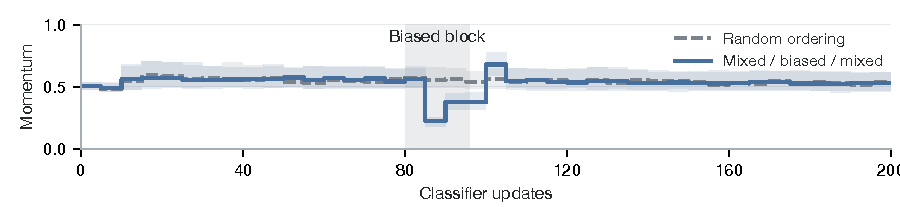
\includegraphics[width=\columnwidth]{figures/momentum_block.pdf}
\caption{Original two-seed SGD momentum response. Gray marks a single-digit block; lines are medians and bands the middle 50\% of 20 episode seeds $\times$ two policy seeds, not confidence intervals. The reactive pattern is descriptive, not evidence of its causal benefit.}
\label{fig:momentum}
\end{figure}

\subsection{Ablations with matched held settings}
\begin{table}[t]
\centering
\caption{Regular all-order accuracy (\%), two training seeds and 20 episode seeds per condition. Restricted controls hold unlearned settings at full-policy starting values. No-feedback removes only the three gradient features; loss and time remain. No CIs are claimed.}
\label{tab:ablation}
\begin{tabular}{lrr}
\toprule
Variant&SGD&Adam\\
\midrule
Full policy&89.44&90.87\\
LR only (start-held)&89.52&89.82\\
LR + WD (start-held memory)&88.83&89.99\\
No gradient features&89.50&89.70\\
\bottomrule
\end{tabular}
\end{table}
The corrected ablations (Table~\ref{tab:ablation}) do not establish a uniform need to control every coordinate. SGD LR-only approximately matches full control, while allowing WD but holding memory is worse. For Adam, both restricted variants trail full control. Earlier tuned-held Adam ablations reached 92.76\% and 92.68\%, but inherited tuned fixed memory settings that the full policy did not receive; those results were an initialization confound, not clean evidence against learned memory control. Removing gradient features leaves SGD competitive but reduces Adam accuracy. This does not remove all feedback, because loss statistics remain available. Figure~\ref{fig:momentum} similarly shows reactivity without isolating its value.

\subsection{Warm-start policies}
Starting from tuned fixed settings yields regular biased means of 90.86\%, 92.69\%, 92.66\%, and 92.63\% for SGD, Adam, AdamW, and RMSprop. Gains over freshly paired fixed controls are +2.51, +1.18, +1.15, and +0.26 pp; all five training seeds beat fixed in each family on this aggregate. Thus adaptive-family underperformance is not intrinsic to the action space: initialization materially changes the outcome. Warm minus original full-policy comparisons match only seeds 338--339, whereas the displayed warm means use five seeds.

On all eight extreme types, including shuffled, warm-minus-fixed gains are +2.32, +2.85, +3.34, and $-0.03$ pp. These are not seven-biased means. SGD warm versus full is $-2.54$ pp on their two matched seeds, so initialization is not uniformly beneficial under distribution shift. There are no bootstrap intervals for this later experiment.

\begin{figure}[t]
\centering
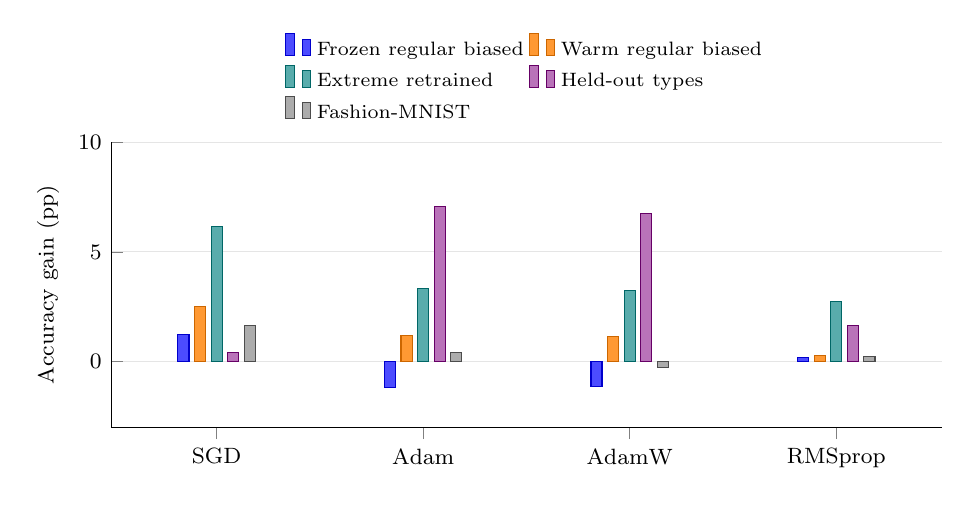
\begin{tikzpicture}
\begin{axis}[
 width=\columnwidth,height=5.2cm,
 ybar,bar width=4pt,
 ymin=-3,ymax=10,
 ylabel={Accuracy gain (pp)},
 symbolic x coords={SGD,Adam,AdamW,RMSprop},xtick=data,
 enlarge x limits=0.17,
 ymajorgrids=true,grid style={gray!20},
 tick label style={font=\footnotesize},label style={font=\footnotesize},
 legend style={font=\scriptsize,at={(0.5,1.03)},anchor=south,legend columns=2,draw=none},
 legend cell align=left,
 axis lines*=left,
 cycle list={{fill=blue!70,draw=blue!80!black},{fill=orange!80,draw=orange!80!black},{fill=teal!65,draw=teal!80!black},{fill=violet!55,draw=violet!80!black},{fill=gray!65,draw=black!70}}
]
\addplot coordinates {(SGD,1.246) (Adam,-1.199) (AdamW,-1.161) (RMSprop,0.202)};
\addplot coordinates {(SGD,2.51) (Adam,1.18) (AdamW,1.15) (RMSprop,0.26)};
\addplot coordinates {(SGD,6.17) (Adam,3.31) (AdamW,3.22) (RMSprop,2.75)};
\addplot coordinates {(SGD,0.39) (Adam,7.06) (AdamW,6.76) (RMSprop,1.64)};
\addplot coordinates {(SGD,1.65) (Adam,0.39) (AdamW,-0.26) (RMSprop,0.21)};
\legend{Frozen regular biased,Warm regular biased,Extreme retrained,Held-out types,Fashion-MNIST}
\end{axis}
\end{tikzpicture}

\caption{Policy-minus-fixed gains (pp), with different evaluation scopes intentionally labeled. Frozen/warm: regular nine-biased means; extreme retrained: seven-biased mean versus extreme-retuned fixed; held-out: all eight types versus fold-retuned fixed; Fashion-MNIST: all ten regular types. Frozen, warm, and retrained use five policy seeds; held-out and Fashion use two. Bars are descriptive, not comparable estimates of one common treatment; no common CI is implied.}
\label{fig:gains}
\end{figure}

\subsection{Retraining on extreme orderings}
Five-seed extreme retraining produces biased means $67.48\pm1.86$\%, $69.22\pm2.81$\%, $69.13\pm3.47$\%, and $72.98\pm1.05$\% (sample SD across seeds). Improvements over extreme-retuned fixed are +6.17, +3.31, +3.22, and +2.75 pp. All seed-matched retrained policies beat their frozen counterparts on the biased aggregate. AdamW seed 341 is the only retrained seed that loses to retuned fixed on this aggregate. Gains are not uniform: all families improve on the half-class block and alternating halves but lose on average on late-single and staircase orderings relative to retuned fixed. Shuffled accuracy drops relative to frozen policies. These are in-distribution adaptation results, because training and test share ordering types, and the five-seed extension has no reported bootstrap CIs.

\subsection{Held-out ordering types}
Leaving out one type at a time gives all-type retrained policy means of 65.15\%, 75.26\%, 75.20\%, and 73.75\%. Relative to fold-retuned fixed, paired gains are $0.39\pm0.37$, $7.06\pm0.33$, $6.76\pm0.33$, and $1.64\pm0.27$ pp, where $\pm$ is one episode-level paired standard error, not a policy-seed SD or 95\% CI. The seven-biased gains are +0.23, +8.08, +7.71, and +1.92 pp. SGD's two policy seeds bracket the all-type fixed result, highlighting training-seed sensitivity.

All four controllers beat every comparator on pair, half-block, sorted, and alternating-half holdouts, but none beat the best comparator on shuffled, late-single, or staircase holdouts. Adam and AdamW remain below 36\% on the sorted holdout despite large relative gains. This tests unseen ordering types, not unrelated shifts: single-max and single-late types, for example, are structurally similar. Conditional episode SEs do not measure uncertainty over new types or new datasets.

\subsection{Fashion-MNIST and CIFAR feasibility}
On Fashion-MNIST, all-order fixed/policy means are 73.89/75.54\% (SGD), 77.33/77.72\% (Adam), 77.81/77.56\% (AdamW), and 78.30/78.51\% (RMSprop). Stored unrounded differences are +1.65, +0.39, $-0.26$, and +0.21 pp. Both training seeds improve for SGD, Adam, and RMSprop; neither does for AdamW. SGD's largest gains occur on repeated-same and three-shock orderings (+4.58 and +3.34 pp). There were no failed test episodes, but only two training seeds, so this remains a small descriptive transfer check.

A CIFAR-10~\cite{krizhevsky2009} timing harness widens the MLP input to 3072, retaining 200 updates and batch 64. Measured episode cost relative to MNIST is $1.37\times$ for SGD and $1.64\times$ for Adam, projecting about 4.3 hours for a full pipeline on the measured VM (a practical budget of 5--7 hours). This uses a 40k/2k/2k split, one timing sample per operation, no warmup, and Adam as a timing proxy for AdamW/RMSprop. A CNN was not timed. No CIFAR accuracy result or large-scale generalization claim follows from this feasibility estimate.

\section{Discussion and Limitations}
The results distinguish three questions: whether a policy reacts, whether that reaction improves a particular evaluation distribution, and whether the learned behavior transfers. Momentum traces answer the first. SGD's frozen biased gains and the paired intervals answer part of the second. Extreme retraining and held-out-type evaluation show that the third depends strongly on what shifts and initial settings the controller experienced. Figure~\ref{fig:gains} summarizes gains but deliberately does not pool these different experimental treatments.

Warm-start results and corrected ablations make initialization a central explanatory variable. Fixed Adam/AdamW start from substantially different memory settings than the original policy. Granting the controller a tuned start reverses the regular adaptive-family gap; holding ablated coordinates at tuned values had previously obscured this issue. Neither observation proves that one initialization is optimal, nor that learned feedback dominates an optimized open-loop schedule. The small, retrospective schedule control and the loss-feedback retained in the feature ablation leave those causal questions open.

Our scope is narrow: five training seeds for major comparisons and two for others; one small MLP; short episodes; MNIST-scale tasks; and a finite set of structured orderings. Extreme failures are retained, with different historical safeguards across optimizer implementations. Baselines are grid-selected, not exhaustively optimized over arbitrary schedules or population strategies. Bootstrap CIs cover saved comparisons, not the later warm-start, start-held ablation, five-seed retraining, or held-out studies. Policy seeds are not interchangeable with independent datasets, and the official test images were used in earlier exploration. New episode seeds therefore do not constitute a fresh test set. Finally, replay drift limits literal row-wise reproducibility even when aggregate trends remain stable; documenting this is preferable to silently relaxing checks or replacing saved evidence.

\balance
\section{Conclusion}
Small feedback-driven policies can improve optimization under biased streams, but benefits depend on optimizer family, starting settings, and training distribution. Frozen SGD improves consistently on the studied biased suites; original Adam/AdamW policies can deteriorate sharply. Tuned warm initialization and extreme-distribution retraining change that picture, while held-out-type results show conditional rather than universal transfer. This is a limited exploration of POMDP-based optimizer control, not a scalable solution to the full optimization decision problem. Stronger evaluation should use new datasets and models, more policy seeds, prospectively fitted schedule controls, and matched initialization and compute before making general claims about learned feedback.

\section*{Contributions}
\textbf{TODO: author contributions}

\printbibliography
\end{document}
